\let\negmedspace\undefined
\let\negthickspace\undefined
\documentclass[journal]{IEEEtran}
\usepackage[a5paper, margin=10mm, onecolumn]{geometry}
%\usepackage{lmodern} % Ensure lmodern is loaded for pdflatex
\usepackage{tfrupee} % Include tfrupee package

\setlength{\headheight}{1cm} % Set the height of the header box
\setlength{\headsep}{0mm}     % Set the distance between the header box and the top of the text

\usepackage{gvv-book}
\usepackage{gvv}
\usepackage{cite}
\usepackage{amsmath,amssymb,amsfonts,amsthm}
\usepackage{algorithmic}
\usepackage{graphicx}
\usepackage{textcomp}
\usepackage{xcolor}
\usepackage{txfonts}
\usepackage{listings}
\usepackage{enumitem}
\usepackage{mathtools}
\usepackage{gensymb}
\usepackage{comment}
\usepackage[breaklinks=true]{hyperref}
\usepackage{tkz-euclide} 
\usepackage{listings}
% \usepackage{gvv}                                        
\def\inputGnumericTable{}                                 
\usepackage[latin1]{inputenc}                                
\usepackage{color}                                            
\usepackage{array}                                            
\usepackage{longtable}                                       
\usepackage{calc}                                             
\usepackage{multirow}                                         
\usepackage{hhline}                                           
\usepackage{ifthen}                                           
\usepackage{lscape}
\begin{document}

\bibliographystyle{IEEEtran}

\title{2.10.52}
\author{EE25BTECH11023 - Venkata Sai}
% \maketitle
% \newpage
% \bigskip
{\let\newpage\relax\maketitle}

\renewcommand{\thefigure}{\theenumi}
\renewcommand{\thetable}{\theenumi}
\setlength{\intextsep}{10pt} % Space between text and floats


\numberwithin{align}{enumi}
\numberwithin{figure}{enumi}
\renewcommand{\thetable}{\theenumi}


\textbf{Question}:\newline
Let $\vec{a} = \hat{\vec{i}} + 2\hat{\vec{j}} + \hat{\vec{k}}$, $\vec{b} = \hat{\vec{i}} - \hat{\vec{j}} + \hat{\vec{k}}$ and $\vec{c} = \hat{\vec{i}} + \hat{\vec{j}} - \hat{\vec{k}}$. A vector in the plane of $\vec{a}$ and $\vec{b}$ whose projection on $\vec{c}$ is $\frac{1}{\sqrt{3}}$, is
\begin{multicols}{4}
\begin{enumerate}
\item 4$\hat{\vec{i}} - \hat{\vec{j}} + 4\hat{\vec{k}}$
\item 3$\hat{\vec{i}} + \hat{\vec{j}} - 3\hat{\vec{k}}$
\item $2\hat{\vec{i}} + \hat{\vec{j}} - 2\hat{\vec{k}}$
\item $4\hat{\vec{i}} + \hat{\vec{j}} - 4\hat{\vec{k}}$
\end{enumerate}
\end{multicols}

\textbf{Solution: }

Given
\begin{align}
\vec{a}=\myvec{1\\2\\1},\vec{b}=\myvec{1\\-1\\1},\vec{c}=\myvec{1\\1\\-1}
\end{align}

Let $\vec{r}$ be coplanar to $\vec{a}$ and $\vec{b}$
\begin{align}
 \vec{r}&=\vec{a}+t\vec{b} 
 \end{align}
Given the projection of $\vec{r}$ on $\vec{c}$ is $\frac{1}{\sqrt{3}}$
\begin{align}
\frac{|\vec{r}^\top\vec{c}|}{\norm{\vec{c}}} = \frac{1}{\sqrt{3}} \\
\implies \vec{r}^\top\vec{c}=\pm\frac{\norm{\vec{c}}}{\sqrt{3}}
\end{align}
\begin{align}
\vec{r}^\top\vec{c}&=\brak{\vec{a}+t\vec{b}}^\top\vec{c}\\
&=\brak{\vec{a}^\top+t\vec{b}^\top}c \\
&=\vec{a}^\top\vec{c}+t\brak{\vec{b}^\top\vec{c}} 
\end{align}
\begin{align}
\vec{r}^\top\vec{c}-\vec{a}^\top\vec{c}=t\brak{\vec{b}^\top\vec{c}}  \\
\implies t=\frac{\vec{r}^\top\vec{c}-\vec{a}^\top\vec{c}}{\vec{b}^\top\vec{c}}
\end{align}
From \brak{2}
\begin{align}
    \vec{r}=\vec{a}+\brak{\frac{\vec{r}^\top\vec{c}-\vec{a}^\top\vec{c}}{\vec{b}^\top\vec{c}}}\vec{b} \\
    \vec{r}=\vec{a}+\brak{\frac{\pm\frac{\norm{\vec{c}}}{\sqrt{3}}-\vec{a}^\top\vec{c}}{\vec{b}^\top\vec{c}}}\vec{b}
\end{align}
\begin{align}
\norm{\vec{c}}^2=\vec{c}^\top\vec{c}&=\myvec{1&1&-1}\myvec{1\\1\\-1} \\
&=1+1+1=3  \implies \norm{\vec{c}}=\sqrt{3}
\end{align}  
\begin{align}
\vec{a}^\top\vec{c}=\myvec{1&2&1}\myvec{1\\1\\-1}=1+2-1=2 
\end{align}
\begin{align}
\vec{b}^\top\vec{c}=\myvec{1&-1&1}\myvec{1\\1\\-1}=1-1-1=-1 \\
\end{align}
Substitute \brak{13},\brak{14},\brak{15} in \brak{11} \\
\begin{align}
\vec{r}=\myvec{1\\2\\1}+\brak{\frac{\pm1-2}{-1}}\myvec{1\\-1\\1} 
\end{align}
\begin{align}
\implies \vec{r}=\myvec{1\\2\\1}+\myvec{1\\-1\\1}\ \text{or}\ \myvec{1\\2\\1}+3\myvec{1\\-1\\1}
\implies \vec{r}=\myvec{2\\1\\2}\ \text{or} \myvec{4\\-1\\4}
\end{align}
Hence Option(1) is the correct answer

\begin{figure}[h!]
   \centering
   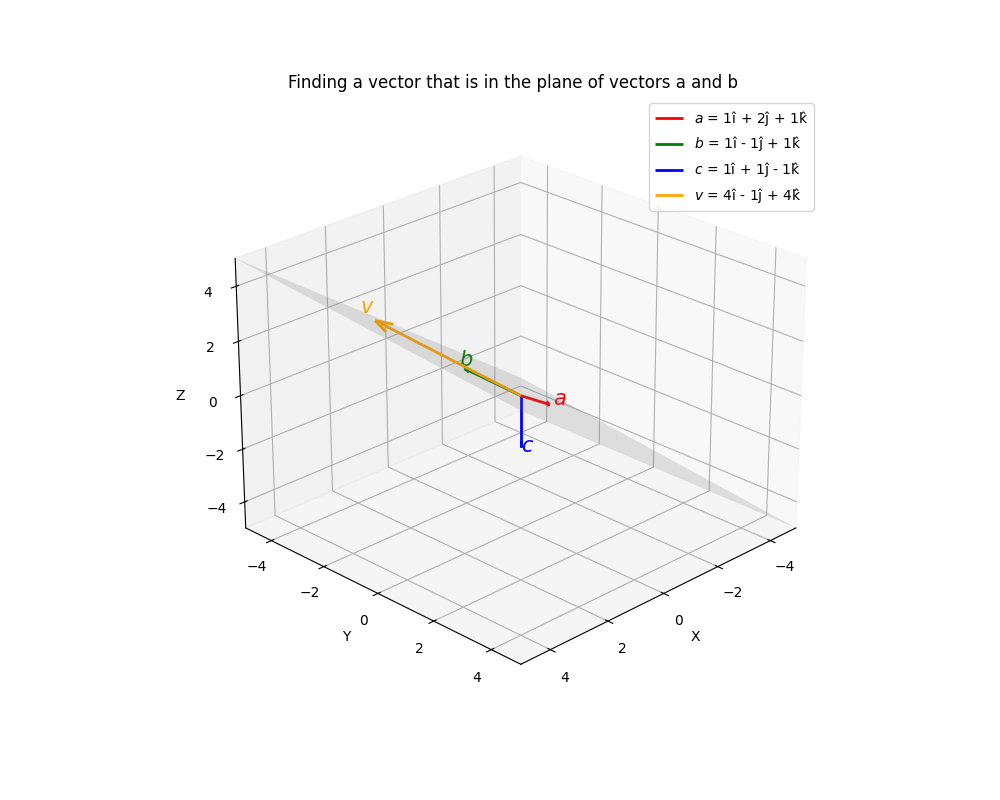
\includegraphics[width=0.7\columnwidth]{figs/fig1.png}
   \caption{}
   \label{Figure}
\end{figure}
\end{document}  
